\chapter{Results and Discussion}

[Write 1 opening paragraph.]

\section{Estimation at unmonitored stations}
% Source: docs/phase1_report.md, section 7.1 (dataset v3). Table of R^2 (RMSE) by split and model.
% Key: no-lag Random Forest R^2 0.41 temporal, 0.31 blocked, 0.32 LOSO, 0.20 combined;
% climatology combined 0.13. Figures: results_pred_vs_obs.png, results_station_spread.png.
% Per-station spread: median 0.22; TN 0.37 ... Telangana -0.22.
[Write.]

\section{Value of satellite inputs}
% Section 7.2: Tier A - Tier B; LOSO +0.020 [+0.009, +0.031]; SW monsoon +0.049 [+0.018, +0.096];
% blocked +0.004 [-0.021, +0.027]; temporal -0.007. Ablation figure results_ablation.png.
[Write.]

\section{Effect of cloud and the monsoon}
% Section 7.3: cloud-bin table; AOD exists on 2,092 of 23,932 cloudiest rows.
% Figures: results_skill_by_cloud.png, eda_aod_vs_cloud.png. Two side-by-side figures example:
\begin{figure}[h]
    \begin{subfigure}[t]{0.48\textwidth}
        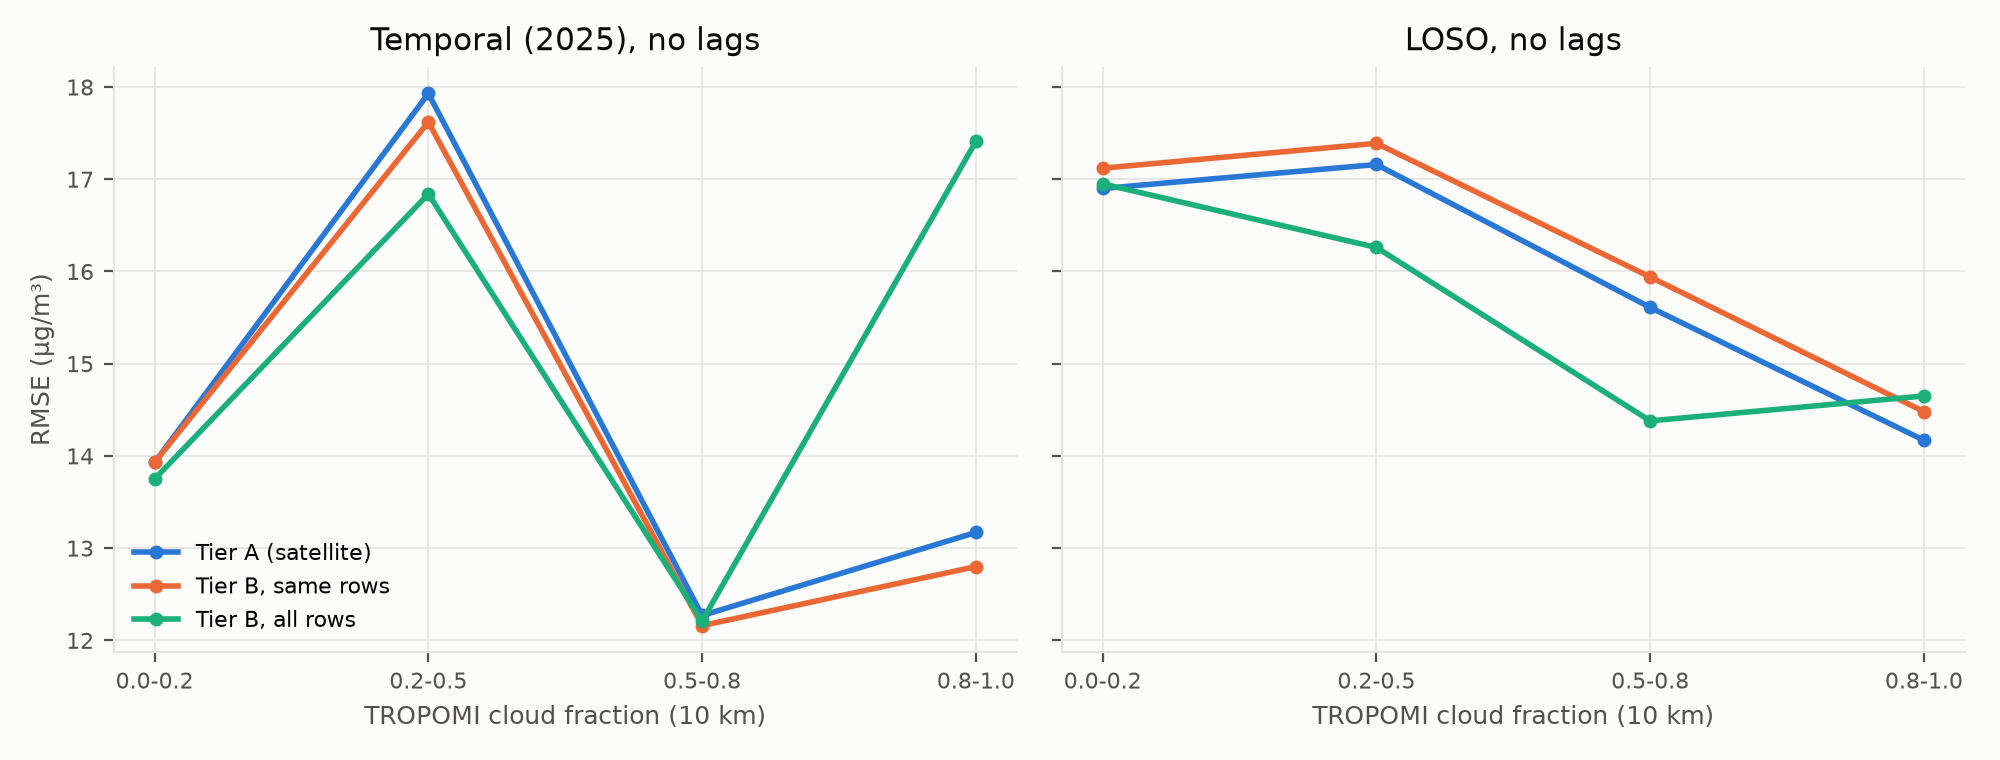
\includegraphics[width=\linewidth]{results_skill_by_cloud}
        \caption{Skill by cloud fraction.}
        \label{fig:skill_cloud}
    \end{subfigure}
\hfill
    \begin{subfigure}[t]{0.48\textwidth}
        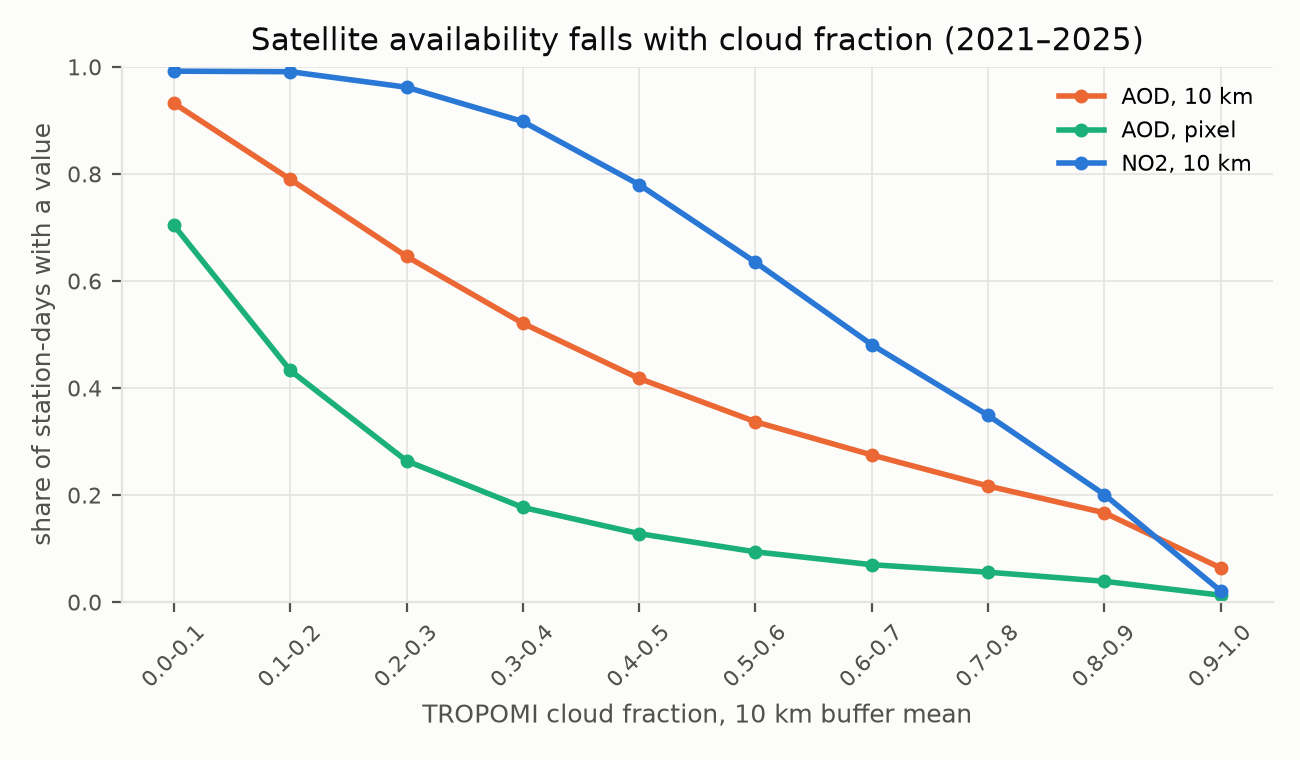
\includegraphics[width=\linewidth]{eda_aod_vs_cloud}
        \caption{AOD availability against cloud fraction.}
        \label{fig:aod_cloud}
    \end{subfigure}
    \caption{Cloud and satellite availability.}
    \label{fig:cloud}
\end{figure}
[Write.]

\section{Two-tier system and sensitivity}
% Sections 7.4-7.5: two-tier over climatology LOSO +0.091 [+0.002, +0.169]; sensitivity table.
[Write.]

\section{Hourly forecasting at existing stations}
% Source: docs/stage6_forecasting.md section 6. Table of R^2 by horizon; figure forecast_r2_by_horizon.png;
% Random Forest best (0.813 / 0.430 / 0.321 at 1 / 24 / 72 h); networks 0.01-0.07 below in every seed;
% satellite adds nothing (Tier A - B -0.007 to +0.001); perfect weather +0.02-0.04 at 72 h.
[Write.]

\section{Comparison with the literature}
% Our 72 h R^2 0.32 vs Qi et al. 0.72 (BTH, long episodes); our "with lags" daily models 0.70-0.76
% match forecasting papers; our LOSO 0.3 answers the harder estimation task.
[Write.]

\section{Limitations}
% phase1_report.md limitations + stage6 section 8 (one RF seed, reanalysis in place of real time, ...).
[Write.]
